\documentclass{beamer}
%% Possible paper sizes: a0, a0b, a1, a2, a3, a4.
%% Possible orientations: portrait, landscape
%% Font sizes can be changed using the scale option.
\usepackage[size=a3,orientation=portrait,scale=1.8]{beamerposter}
\usetheme{LLT-poster}
\usecolortheme{ComingClean}

%\usecolortheme{Entrepreneur}
%\usecolortheme{ConspiciousCreep}  %% VERY garish.
\usepackage{eurosym}
\usepackage[utf8]{inputenc}
\usepackage[T1]{fontenc}
\usepackage{libertine}
\usepackage[scaled=0.92]{inconsolata}
\usepackage[libertine]{newtxmath}
\usepackage[numbers]{natbib}
\renewcommand{\bibfont}{\small}

\newcommand{\texthash}{\#}


%% Load the markdown package
\usepackage[citations,footnotes,definitionLists,hashEnumerators,smartEllipses,tightLists=false,pipeTables,tableCaptions,hybrid]{markdown}
%%begin novalidate
\markdownSetup{rendererPrototypes={
 link = {\href{#2}{#1}},
 headingFour = {\begin{block}{#1}},
 horizontalRule = {\end{block}}
}}
%%end novalidate

\author[Chevalier.V]{mecacorbu.odoo.com/}
\title{STS CPRP $2^{eme}$ année}
\institute{Lycée Le Corbusier}
% Optional foot image
\footimage{
\includegraphics[width=4cm]{logo1.png}}

\begin{document}

\begin{frame}[fragile]\centering

\textbf{\textit{Résumé - Seuil de rentabilité}}

\begin{columns}
\begin{column}{0.57\textwidth}

\begin{markdown}

#### Rappels mathématiques

- On appelle \textit{fonction affine} une fonction de type : $y=a.x+b$
- On peut tracer plusieurs fonctions affines sur un même graphe pour les comparer
- $y$ : L'ordonnée. Dans notre cas : le coût/prix du procédé qu'on cherche à comparer avec un autre. Aussi noté "$P$" (procédé) dans les exercices
- $a$ : coefficient directeur, ou l'angle par rapport à l'abscisse. Dans notre cas : le coût de revient pour sortir une ou plusieurs pièces (ex : panoplie)
- $x$ : la valeur qui varie, dans notre cas : \textbf{le nombre de pièce à usiner}, aussi noté $n$ dans les exercices.
- $b$ : L'ordonnée à l'origine (si $b \neq 0$, la fonction ne passera pas par zéro), dans notre cas : les dépenses fixes, en plus de l'usinage et qu'on cherche souvent à amortir (prix d'un moule, achat d'une nouvelle MOCN, automatisation d'une chaîne de production, etc.)



----
\end{markdown}

\end{column}




\begin{column}{.4\textwidth}
\begin{markdown}




#### Exemple type

- Après consultation de spécialistes de chaque domaine, nous avons obtenu les chiffrages suivant :
- Obtention des pièces par usinage : coût de 3\euro par pièce intégrant la part d’investissement matériel et matière ;
- Obtention des pièces par injection plastique : coût d'un moule 3000\euro, coût de revient d’un cycle d’injection 0,5\euro par grappe de deux pièces intégrant le coût de réglage de la presse.
- Question: \textbf{Déterminer} la zone de rentabilité de chaque procédé \textit{graphiquement} ou \textit{analytiquement} en détaillant vos calculs.
\textbf{Conclure} sur le procédé à utiliser pour réaliser 2 000 pièces d'une PME.

----
\end{markdown}


\end{column}

\end{columns}

\bigskip

\textbf{\textit{Résolution analytique}}

\bigskip
    
\begin{columns}[T]

%%%% First Column
\begin{column}{.46\textwidth}

\begin{markdown}

#### 1. Données 

- On prend toutes nos données pour avoir une fonction de type $y=a.x+b$
- Usinage, Procédé 1 :  $P_1= a. x + b = 3.x + 0$
- Injection, Procédé 2 :  $P_2= a. x + b = \frac{0.5}{2}.x + 3000$

----


#### 3. Quel procédé choisir ?

- On veut savoir quel procédé est le moins cher pour 15000 pièces
- Pièces $=2000 = x $, on trouve les deux $y$ avec $P1$ et $P2$
- $P1=3 \times 2000 =$ 6 000 \euro
- $P2=\frac{0.5}{2} \times 2000 + 3000 =$ 3 500 \euro


\setkeys{Gin}{width=.3\linewidth}



----


\end{markdown}



\end{column}









%%%% Second Column
\begin{column}{.46\textwidth}

\begin{markdown}

#### 2. Déterminer - Zone de rentabilité

- Ici, P1 et P2 sont deux fonctions affines 
- Trouver l'intersection des fonctions revient à résoudre l'équation $P1(x) = P2(x)$
- $y=3.x$ et $y=\frac{0.5}{2}.x+3000$
- $3.x=\frac{0.5}{2}.x+3000$
- $3.x-\frac{0.5}{2}.x=3000$
- $(3-0.25).x = 3000 \Leftrightarrow 2.75.x =3000$
- $x=\frac{3000}{2.75} \Leftrightarrow x \simeq 1091$ pièces



----


\end{markdown}
\end{column}
\end{columns}


\bigskip
{\usebeamercolor[bg]{headline}\hrulefill}
\bigskip

\begin{markdown}

#### 4. Conclusion

- On a calculé que pour usiner 2 000 pièces, le procédé d'injection plastique est moins cher. 
- Le seuil de rentabilité se situe à 1091 pièces, avant il est plus rentable d'utiliser l'usinage. Si la commande est supérieur à 1091 pièces, on privilégiera l'injection plastique.

----

\end{markdown}

\end{frame}











\begin{frame}[fragile]\centering

\textbf{\textit{résolution graphique}}

\begin{columns}
\begin{column}{0.57\textwidth}

\begin{markdown}

#### 1. Données

- On écrit les deux fonctions :
- $y_1 = 3.x$
- $y_2 = \frac{0.5}{2}.x+3000$



----
\end{markdown}

\end{column}




\begin{column}{.4\textwidth}
\begin{markdown}




#### 2. Choisir l'échelle

- Abscisse $\equiv$ nombre de pièce $\simeq$ 2 000 max
- Ordonnées $\equiv$ coût $\simeq$ prévoir large, ici au moins 3000 car $y_2$ sera supérieur à 3000 \euro.
- Il est fort probable de faire une erreur d'échelle, si on a prévu trop petit, on recommence.

----
\end{markdown}


\end{column}

\end{columns}

\bigskip

\begin{markdown}

#### 3. Tracer les deux fonctions

- On trouve deux points par procédé (par fonction)
- Ici on peut prendre par exemple $x=500$ puis $x=1500$
- $P1(500)=3\times 500 = 1500$ et $P1(1500)=3\times 1500=4500$
- $P2(500)=\frac{0.5}{2}\times 500 + 3000 = 3125$ et $P2(1500)=\frac{0.5}{2}\times 1500 + 3000=3375$ 
- 500 et 1500 représentent $x$, le nombre de pièce, les résultats représentent $y$, le prix.

----

\end{markdown}




\bigskip

\begin{figure}
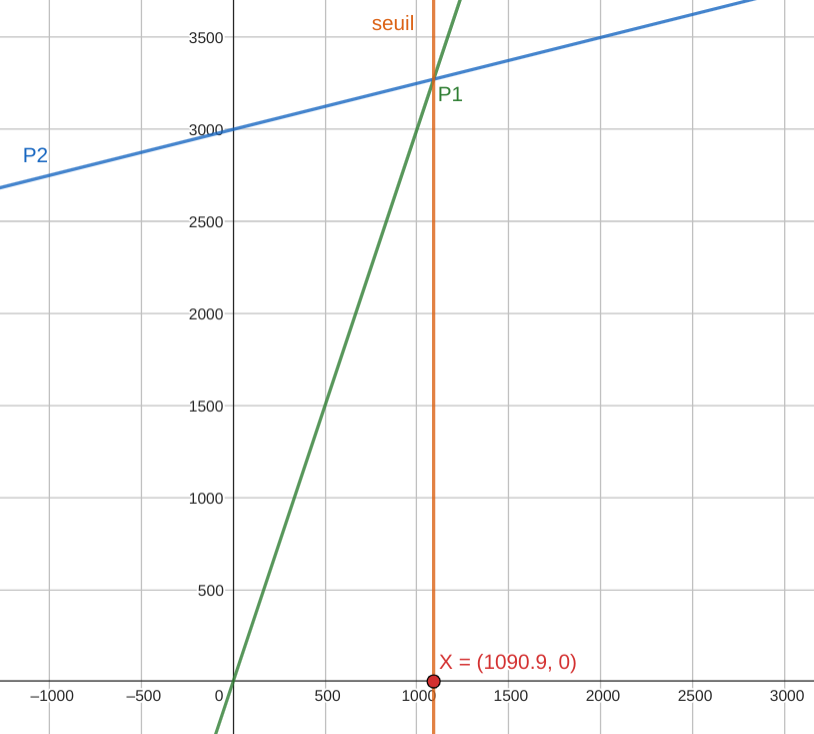
\includegraphics[width=0.7\textwidth]{G2.png}
\caption{Tracé des deux procédés avec \textit{Géogébra}}
\end{figure}

\bigskip




\bigskip

\begin{markdown}

#### 4. Conclusion

- Une fois le graphique tracé, on lis que le seuil est à $\simeq$ 1091 pièces. Et que passé ce seuil de 1091 pièces, il sera préférable de choisir le procédé par injection plastique.

----

\end{markdown}

\end{frame}

















\end{document}